\documentclass[tikz,border=6pt]{standalone}
\usepackage[T1]{fontenc}
\usepackage[utf8]{inputenc}
\usepackage{amsmath,amssymb}
\usepackage{graphicx}
\usepackage{xcolor}
\usepackage{tikz}
\usepackage{pgfplots}
\usetikzlibrary{arrows.meta,backgrounds,calc,fit,matrix,positioning,shapes.geometric,shapes.misc}
\pgfplotsset{compat=1.18}

\definecolor{ink}{HTML}{1F2A30}
\definecolor{slate}{HTML}{5C6A73}
\definecolor{teal}{HTML}{2B7A8C}
\definecolor{brick}{HTML}{B6514A}
\definecolor{gold}{HTML}{C9951A}
\definecolor{sage}{HTML}{6B8C6E}
\definecolor{sky}{HTML}{5E8CC0}
\definecolor{paperbg}{HTML}{FBF7EF}
\definecolor{panel}{HTML}{F2ECE2}
\definecolor{linegray}{HTML}{D4CBBE}
\definecolor{softgreen}{HTML}{DCEBD8}
\definecolor{softred}{HTML}{F4DAD5}
\definecolor{softblue}{HTML}{DCE8F4}
\definecolor{softgold}{HTML}{F4E7C6}

\tikzset{
  figtitle/.style={font=\bfseries\Large, text=ink},
  flowbox/.style={
    draw=ink,
    rounded corners=6pt,
    line width=0.9pt,
    fill=paperbg,
    minimum height=1.35cm,
    minimum width=3.1cm,
    align=center,
    text=ink,
    inner sep=7pt
  },
  sourcebox/.style={flowbox, fill=softblue, draw=sky},
  missingbox/.style={flowbox, fill=softred, draw=brick, dashed},
  gatebox/.style={flowbox, fill=softgold, draw=gold!90!ink, text width=3.7cm},
  successbox/.style={flowbox, fill=softgreen, draw=sage, text width=3.8cm},
  card/.style={
    draw=ink,
    rounded corners=6pt,
    line width=0.8pt,
    fill=paperbg,
    text=ink,
    text width=4.0cm,
    align=left,
    inner sep=7pt
  },
  promote/.style={card, fill=softgreen, draw=sage},
  hold/.style={card, fill=softgold, draw=gold!80!ink},
  retire/.style={card, fill=softred, draw=brick},
  headercard/.style={
    draw=ink,
    rounded corners=7pt,
    line width=1.0pt,
    fill=panel,
    text=ink,
    font=\bfseries\large,
    minimum width=4.3cm,
    minimum height=1.0cm,
    align=center
  },
  figarrow/.style={-Latex, line width=1.05pt, draw=slate},
  stagearrow/.style={-Latex, line width=1.2pt, draw=ink},
  faintarrow/.style={-Latex, line width=0.9pt, draw=linegray},
  ann/.style={font=\footnotesize, text=slate, align=left},
  smallann/.style={font=\scriptsize, text=slate, align=left},
  metric/.style={
    draw=ink,
    rounded corners=6pt,
    line width=0.8pt,
    fill=white,
    text=ink,
    text width=3.6cm,
    align=left,
    inner sep=7pt
  },
  legendlabel/.style={font=\small, text=ink}
}

\pgfplotsset{
  archivara axis/.style={
    width=15cm,
    height=8.6cm,
    axis line style={draw=ink, line width=0.9pt},
    tick style={draw=ink},
    ticklabel style={font=\small, text=ink},
    label style={font=\small, text=ink},
    grid=both,
    major grid style={draw=linegray, line width=0.35pt},
    minor grid style={draw=linegray!60, line width=0.2pt},
    legend style={
      draw=none,
      fill=none,
      font=\small,
      text=ink,
      /tikz/every even column/.append style={column sep=0.5cm}
    },
    clip=false
  }
}


\begin{document}
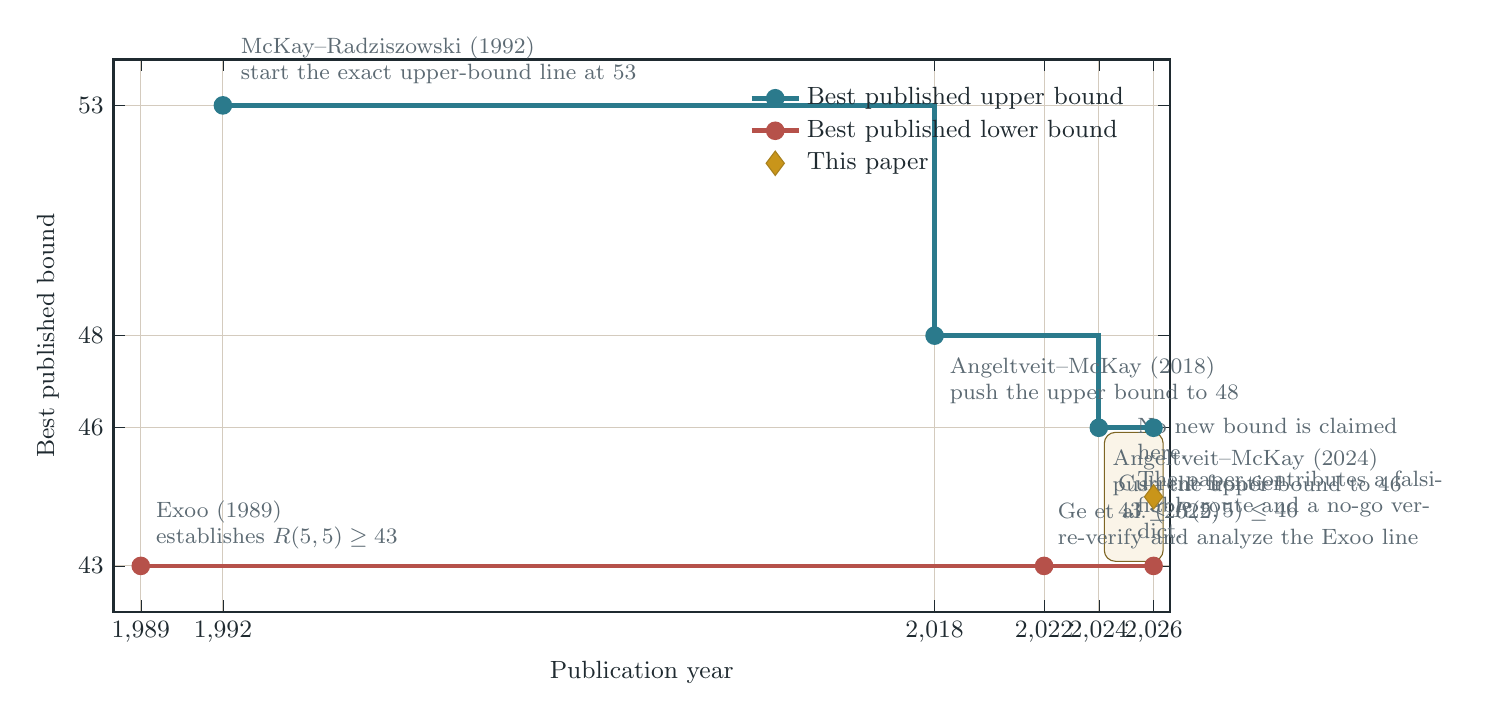
\begin{tikzpicture}
  \begin{axis}[
    archivara axis,
    xmin=1988, xmax=2026.6,
    ymin=42, ymax=54,
    xlabel={Publication year},
    ylabel={Best published bound},
    xtick={1989,1992,2018,2022,2024,2026},
    ytick={43,46,48,53},
    legend cell align=left,
    legend pos=north east
  ]
    \path[fill=gold!10, draw=gold!55!ink, rounded corners=4pt]
      (axis cs:2024.2,43.1) rectangle (axis cs:2026.35,45.9);

    \addplot[
      draw=teal,
      line width=1.7pt,
      const plot,
      mark=*,
      mark size=2.5pt,
      mark options={fill=teal, draw=teal}
    ] coordinates {
      (1992,53)
      (2018,48)
      (2024,46)
      (2026,46)
    };
    \addlegendentry{Best published upper bound}

    \addplot[
      draw=brick,
      line width=1.7pt,
      mark=*,
      mark size=2.5pt,
      mark options={fill=brick, draw=brick}
    ] coordinates {
      (1989,43)
      (2022,43)
      (2026,43)
    };
    \addlegendentry{Best published lower bound}

    \addplot[
      only marks,
      mark=diamond*,
      mark size=4.4pt,
      mark options={fill=gold, draw=gold!80!ink}
    ] coordinates {(2026,44.5)};
    \addlegendentry{This paper}

    \node[ann, anchor=south west] at (axis cs:1989.2,43.15)
      {Exoo (1989)\\establishes $R(5,5)\ge 43$};
    \node[ann, anchor=south west] at (axis cs:2022.15,43.15)
      {Ge et al.\ (2022)\\re-verify and analyze the Exoo line};
    \node[ann, anchor=south west] at (axis cs:1992.3,53.25)
      {McKay--Radziszowski (1992)\\start the exact upper-bound line at $53$};
    \node[ann, anchor=north west] at (axis cs:2018.2,47.75)
      {Angeltveit--McKay (2018)\\push the upper bound to $48$};
    \node[ann, anchor=north west] at (axis cs:2024.15,45.75)
      {Angeltveit--McKay (2024)\\push the upper bound to $46$};
    \node[ann, anchor=west, text width=3.6cm] at (axis cs:2024.35,44.45)
      {Current frontier\\$43 \le R(5,5)\le 46$};
    \node[ann, anchor=west, text width=4.0cm] at (axis cs:2025.05,44.9)
      {No new bound is claimed here.\\The paper contributes a falsifiable route and a no-go verdict.};
  \end{axis}
\end{tikzpicture}
\end{document}
